\section{Experiment}
\label{sec:experiment}

In this section, we show how to model a wheeled-robot controller in \lang{} and generate Arduino C code through our code generator. The generated platform-dependent code has been directly compiled and flashed to the motherboard, without any manual modification.

The hardware platform being used is based on an Arduino Uno motherboard, which consists of 4 motors (divided into two group \em{left} and \em{right}) and an ultrasonic distance sensor, as shown in Fig.~\ref{img:circuits}.

\begin{figure}[!ht]
    \centering
    % \begin{minipage}[t]{0.4\linewidth}
        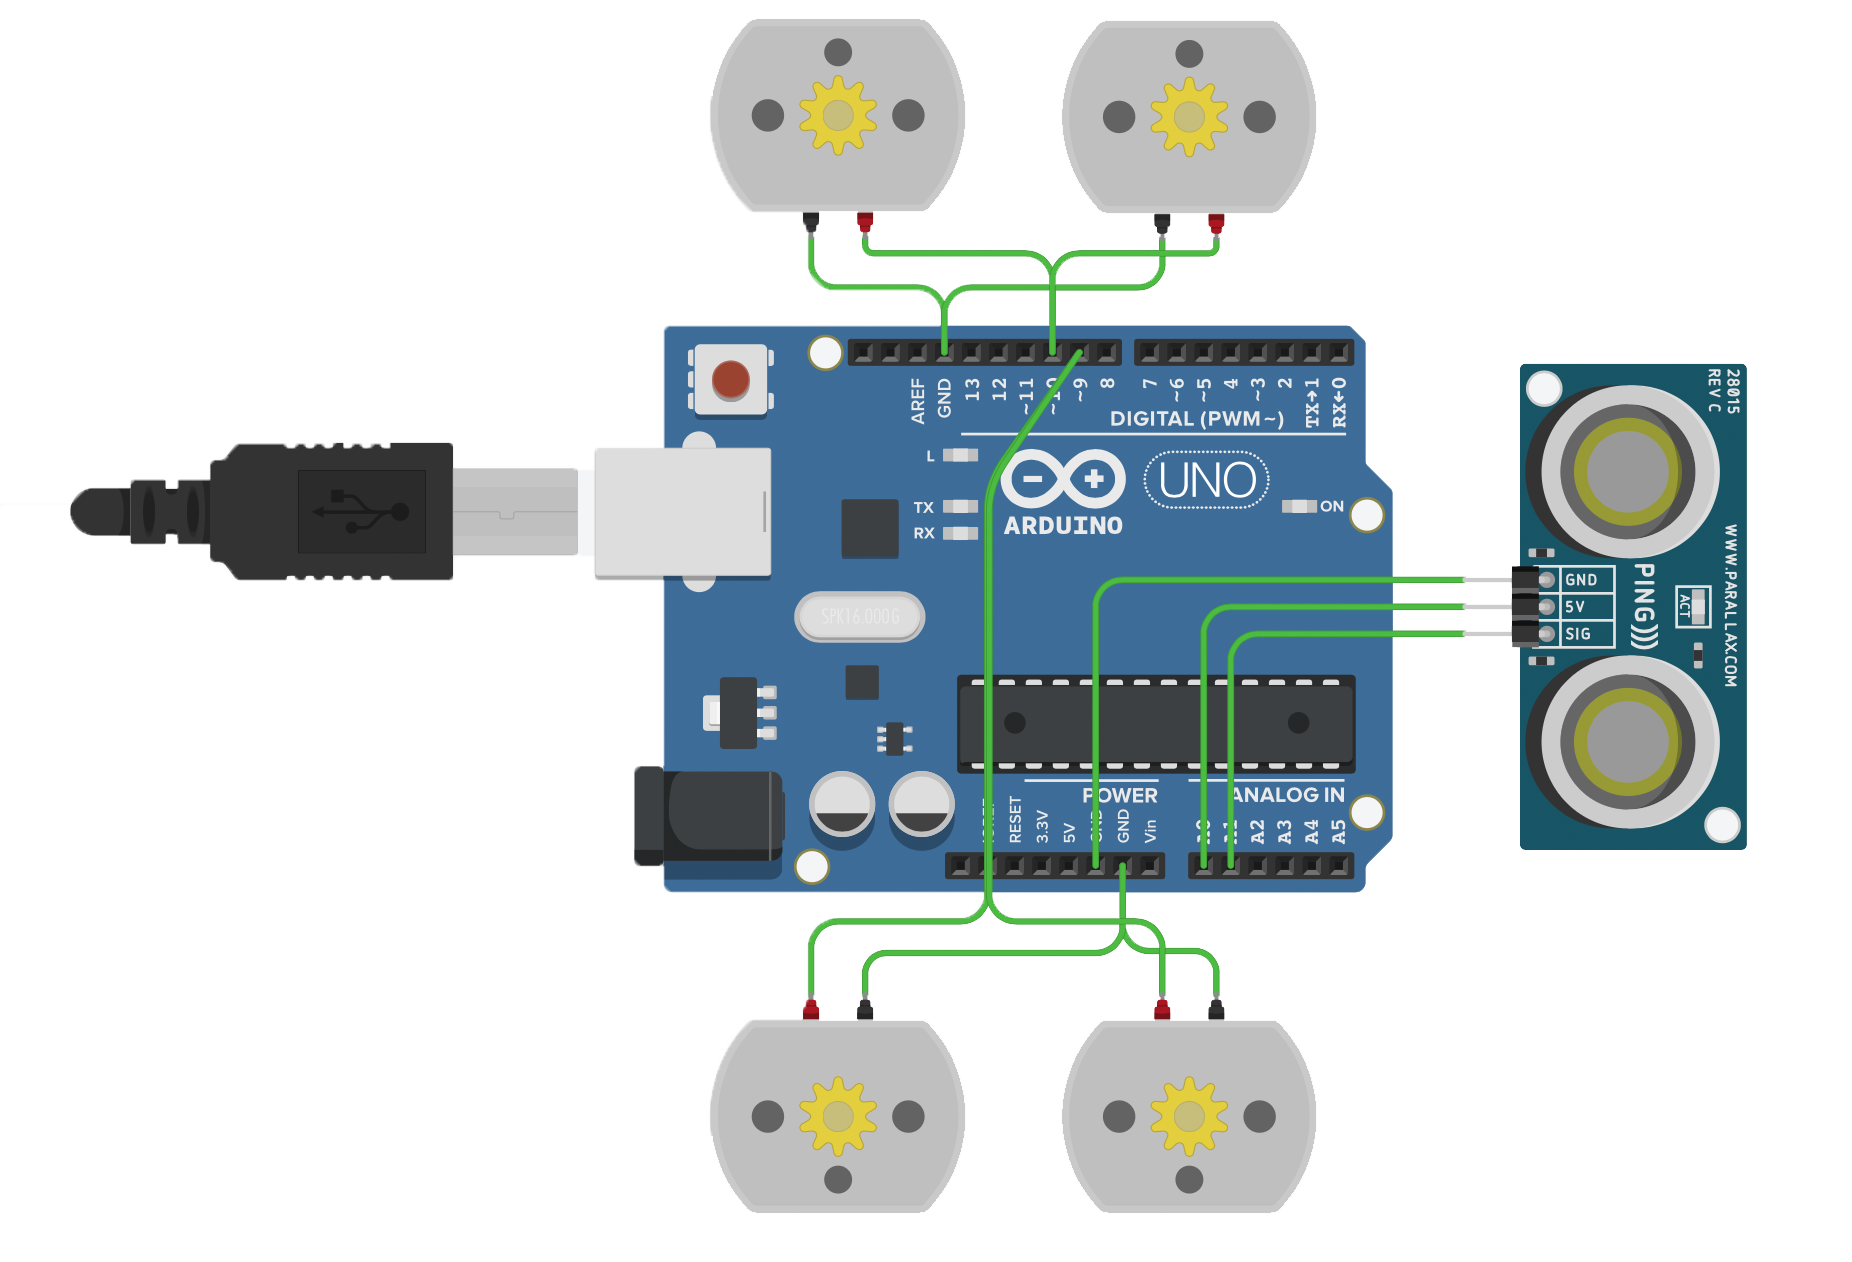
\includegraphics[width=.5\textwidth]{images/circuits.png}
    % \end{minipage}
    % \begin{minipage}[t]{0.4\linewidth}
        % 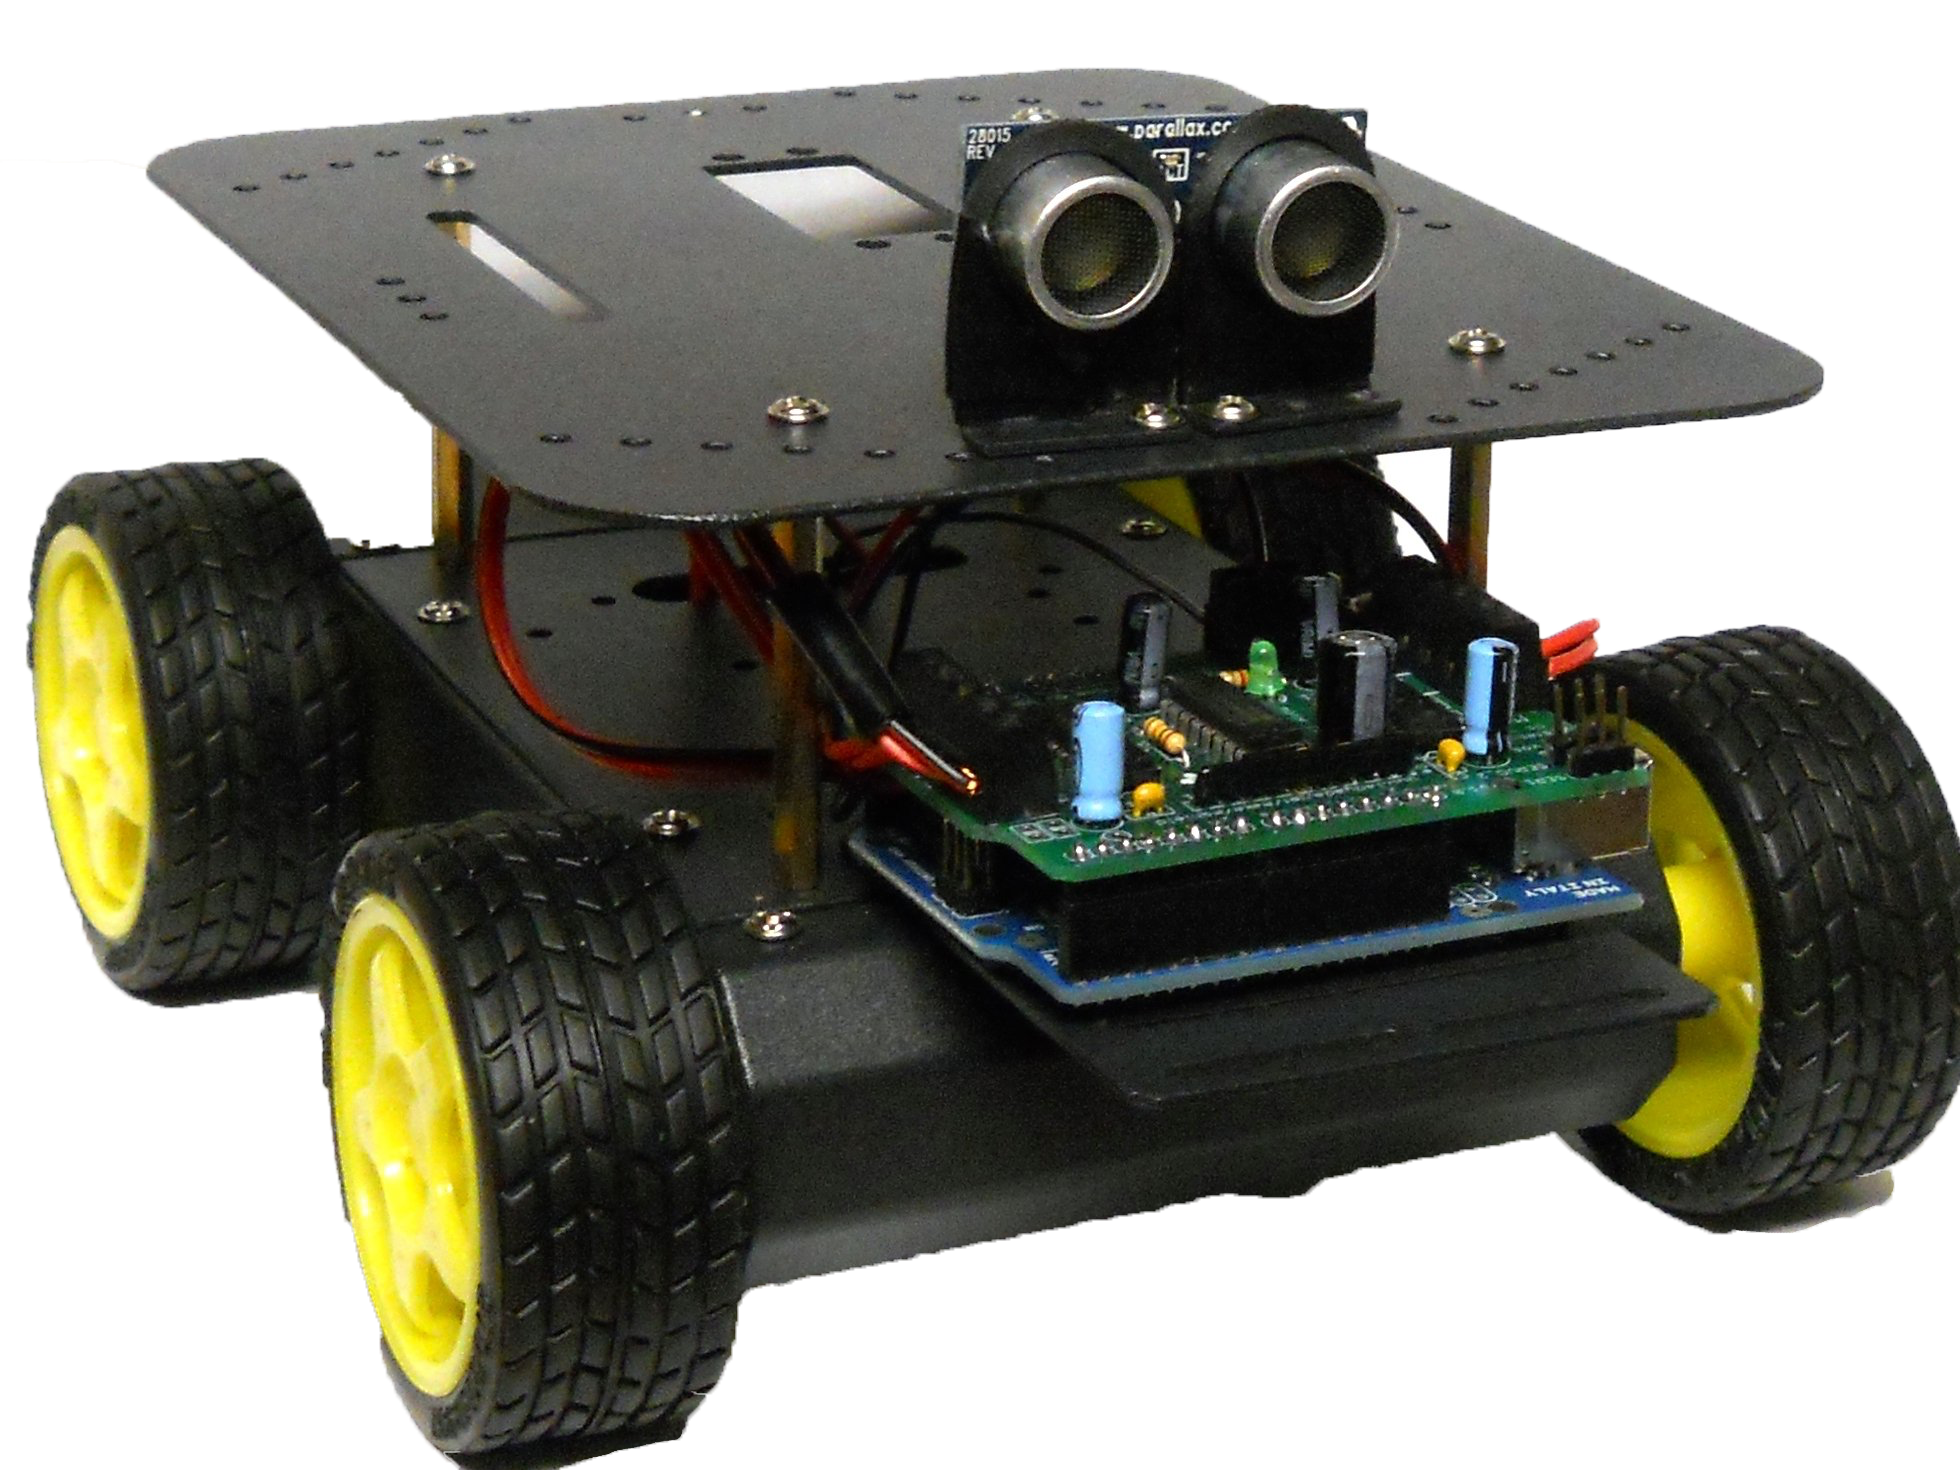
\includegraphics[width=.9\textwidth]{images/robot.png}
    % \end{minipage}
    \caption{Hardware Architecture of the Experiment Platform}
    \label{img:circuits}
\end{figure}

%\subsection{Formal Model in \lang{}}

The \lang{} model of the wheeled-robot controller as shown in Figure \ref{img:controller} contains the following parts:

\begin{itemize}
    \item \emph{UltraSonic}. This sensor detects the distance from nearest obstacles and sends the distance information to the controller.
    \item \emph{Controller}. The core algorithm of this robot is encapsulated in the controller. It reads distance information from the ultrasonic sensor, and gives an abstract command (e.g. forward, backward, turn, stop) to the \emph{speeder} according to the distance information.
    \item \emph{Speeder}. This automaton updates the speed of two motor groups according to the abstract command it receives from the \emph{controller}.
    \item \emph{Motors}. 4 motors, divided into two groups, are equipped in this small robot. Each motor has two control pins, one for direction and the other for speed. The \lang{} automaton shown in Example \ref{exp:automaton} is the driver for motors. It receives a single control signal \emph{speed} and updates the electronic level of control pins correspondingly.
\end{itemize}

\begin{figure}[ht]
    \centering
    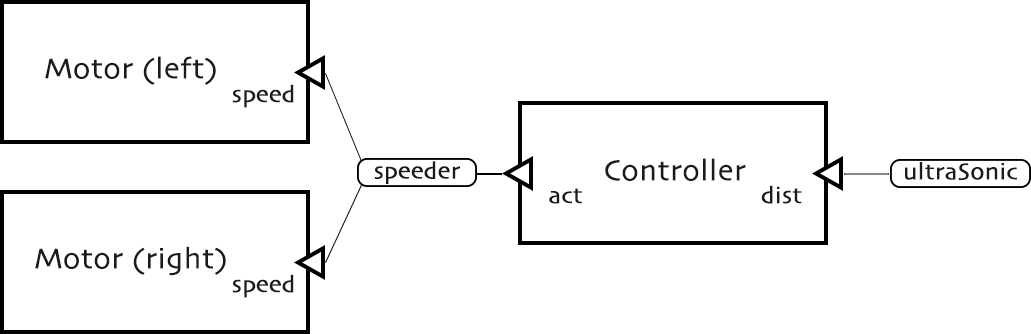
\includegraphics[width=.8\textwidth]{images/architecture.png}
    \caption{Mediator Model of the Robot Controller}
    \label{img:controller}
\end{figure}

%\begin{example}[Robot Controller] 
The controller shown in Figure \ref{img:controller} is captured by the following \lang{} code, where the motors and the controller are defined as components, and the speeder and ultrasonic distance sensor are defined as connections.
    \label{exp:system}
\begin{lstlisting}
system robot () {
    components {
        left_motor : motor<8, 9>;
        right_motor : motor<11, 10>;
        c  : controller;
    }
    connections {
        speeder(c.act, left_motor.speed, right_motor.speed);
        ultraSonicDist<6,7>(c.dist);
    }
}
\end{lstlisting}
%\end{example}

Four \lang{} automata are specified in this controller model: \emph{motor}, \emph{controller}, \emph{speeder} and \emph{ultraSonicDist}. Here we only show the definition of \emph{motor}, further details can be found at \cite{medgit}.

%\begin{example}[Motor Driver]
%    \label{exp:automaton}
    A typical driver of motors with two control signals is defined as an automaton in \lang{}. The simple automaton contains no local variable, one internal transition and one external transition. The internal transition updates the status of port \texttt{speed}, which is supposed to be ready to accept control commands at anytime. And the external transition receives target speed from the \texttt{speed} port and gives orders to the hardware correspondingly. The two template parameters describe where Arduino pins the motor is connected.
    \begin{lstlisting}
automaton <pinDirection,pinSpeed:int> motor (speed:in signedPWM) {
    variables {}
    transitions {
        !speed.reqRead -> speed.reqRead = true; // internal
        speed.reqRead && speed.reqWrite -> {
            sync speed; // external communication flag
            if (speed.value > 0) {
                digitalWrite(pinDirection, 1);
                analogWrite(pinSpeed, speed.value);
            } else {
                digitalWrite(pinDirection, 0);
                analogWrite(pinSpeed, -speed.value);
            }
        }
    }
}
    \end{lstlisting}
%\end{example}

%\subsection{Generated C Codes}

Due to the length limitation, the generated program is omitted here and can be found at \url{https://github.com/mediator-team/codegen-proposal/experiment}.